\documentclass[a4,12pt]{scrartcl}

%Basic 
\usepackage[utf8]{inputenc}
\usepackage[ngerman]{babel}
\usepackage[T1]{fontenc}
\usepackage{float}
\usepackage[bottom = 3.50cm]{geometry}

%Titel Seite
\title{CLOUD INFRASTRUCTURE}
\subtitle{Lab-xx}
\author{Giorgio Vincenti \and Samuel Krieg}
\date{\today}


%Kopf, Fusszeile
\usepackage{fancyhdr}
\pagestyle{fancy}
\lhead{ \begin{picture}(0,0) \put(0,0){
\includegraphics[width=3cm]{./pictures/hsrlogo.png}} \end{picture}}
\chead{}
\rhead{Seite \thepage}
\lfoot{Cloud Infrastructure \\Lab-xx}
\cfoot{Giorgio Vincenti \and Samuel Krieg}
\rfoot{\today}
\renewcommand{\headrulewidth}{0.4pt}

%Bilder
\usepackage{graphicx}

%Tabellen
\usepackage{booktabs}

%Codesnippets
\usepackage{listings}
\lstset{language=bash} 

%Querformat für eine Seite
\usepackage{lscape}
\usepackage{rotating}
\usepackage{pdflscape}

%Temp
\usepackage{lipsum}



\begin{document}

\clearpage\maketitle
\thispagestyle{empty}
\tableofcontents
\newpage

\section{Section}
Text


\subsection{Subsection}
Text


\subsubsection{Subsubsection}
Text

\section{Aufzählung}
\subsection{Itemize}
\begin{itemize}
\item Das erste Item
\item Das zweite Item
\begin{itemize}
\item Das erste Item
\item Das zweite Item
\item Das dritte Item
\end{itemize}
\item Das dritte Item
\end{itemize}

\subsection{Enumerate}
\begin{enumerate}
  \item The first item
  \item The second item
  \item The third etc \ldots
\end{enumerate}

\subsection{Description}
\begin{description}
  \item[First] The first item
  \item[Second] The second item
  \item[Third] The third etc \ldots
\end{description}
\begin{description}
  \item[First] \hfill \\
  The first item
  \item[Second] \hfill \\
  The second item
  \item[Third] \hfill \\
  The third etc \ldots
\end{description}

\section{Tabellen}
\begin{center}
    \begin{tabular}{@{} l l r@{}}\toprule    
    {Stockwerk} & {Hostname} & {Anzahl Ports}\\ \midrule
    1 & DataCSW01 & 12\\ \addlinespace
    & DataCSW03 & 12\\ \addlinespace
    & DataCSW04 & 12\\ \addlinespace
    2& DataCSW02 & 24\\
    \bottomrule
    \end{tabular}
\end{center}

\section{Codesnippets}
\begin{lstlisting}
sudo apt-get install qemu
\end{lstlisting}

\section{Bilder}
\begin{figure} [H]
	\begin{center}
	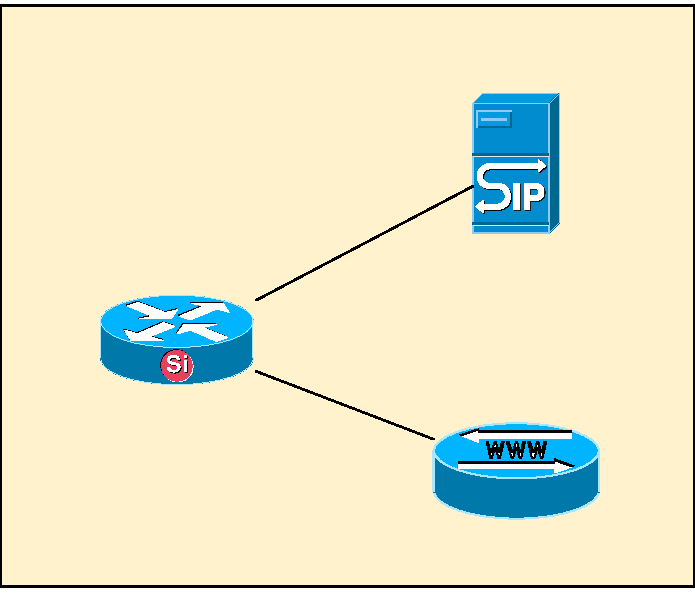
\includegraphics[width=0.50\textwidth]{./pictures/sample_picture.pdf}
	\caption{\textbf{Bild Unterschrift}}
	\label{Bild Referenz}
	\end{center}
\end{figure}

\begin{landscape}
\begin{figure}[htbp]
\subsection{Querformat}
\centering
\fbox{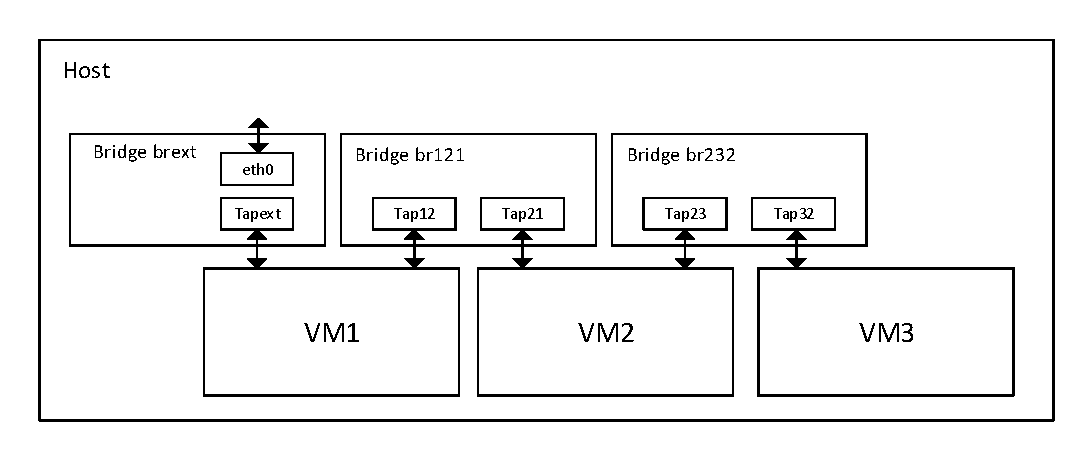
\includegraphics[width=\linewidth, height=\textheight,keepaspectratio]{./pictures/sample_picture_landscape.pdf}}
\caption{\textbf{Bild Querformat}}
\end{figure}
\end{landscape}	


\end{document}
